\chapter{Predicción de abandono en el trabajo}

La empresa me solicitó realizar un prototipo que, partiendo de los datos de una plantilla de trabajadores, fuese capaz de predecir futuros casos de abandono en el trabajo.
Tras su dessarrollo se verían las posibilidades de integrarlo con \wday{}.\\

En este capítulo explicaremos en detalle los datos que vamos a utilizar. Estudiaremos estos datos y construiremos un modelo capaz de predecir cuando un trabajador va a abandonar el trabajo.\\




También se ha usado las librerías \textit{pandas}\footnote{\url{http://pandas.pydata.org/}} para la transformación y análisis de datos y la librería \textit{matplotlib}\footnote{\url{https://matplotlib.org/}} para la visualización de los datos.\\







\section{Datos y problema a resolver}

Se ha realizado un estudio usando los datos con los que cuenta el proyecto de \textit{IBM}, \textit{Watson Analytics}\footnote{Fuente de datos proyecto de \textit{IBM} de \textit{Watson Analytics} \url{https://www.ibm.com/communities/analytics/watson-analytics-blog/hr-employee-attrition/} [Internet; descargado 4-junio-2017]}.
Se trata de una tabla con información sobre los empleados de una empresa.
Estos datos pertenecen a \textit{IBM} y son los que usan para las predicciones analíticas del robot de \textit{Inteligencia artificial} \textit{Watson}. \textit{IBM} ha desarrollado una solución al problema que queremos resolver, pero este proyecto de \textit{IBM} no es de código abierto.\\

Para el uso de los datos he descargado la hoja de cálculo y así poder trabajar localmente.
Después la he convertido a \acrshort{csv} para poder manejar los datos de manera cómoda desde \textit{python}.\\


Se trata de una única tabla, donde cada fila hace referencia a la información de un empleado y donde cada columna nos da información sobre una característica.\\

Hay un total de 1470 empleados (filas) con 35 características (columnas).\\

Algunas de las características con las que contamos son las siguientes:
\begin{itemize}
\item \textbf{Age}: \textit{Número}. indicando la edad.
\item \textbf{Attrition}: \textit{Texto}. indicando si ha abandonado el trabajo o no.
\item \textbf{BusinessTravel}: \textit{Texto}. indicando la frecuencia con la que viaja.
\item \textbf{DailyRate}: \textit{Número}. indicando la tasa diaria del trabajador.
\item \textbf{Department}: \textit{Texto}. con el departamento al que pertenece el empleado.
\item \textbf{DistanceFromHome}: \textit{Número}. con la distancia de casa al trabajo.
\item \textbf{Education}: \textit{Número}. indicando el nivel de educación
\item \textbf{EducationField}: \textit{Texto}. con la rama de educación del trabajador.
\item \textbf{EmployeeCount}: \textit{Número}. que siempre es uno.
\item \textbf{EmployeeNumber}: \textit{Número}. que etiqueta con un identificador a cada empleado.
\item \textbf{EnvironmentSatisfaction}: \textit{Número}. que indica el nivel de satisfacción del trabajador.
\item \textbf{Gender}: \textit{Texto}. especificando el género
\item \textbf{HourlyRate}: \textit{Número}. indicando la tasa por hora del empleado.
\item \textbf{JobInvolvement}: \textit{Número}. indicando el grado de involucración en el trabajo.
\item \textbf{JobLevel}: \textit{Número}. especificando el nivel en el trabajo.
\item \textbf{JobRole}: \textit{Texto}. indicando el puesto de trabajo del empleado.
\item \textbf{JobSatisfaction}: \textit{Número}. especificando el nivel de satisfacción
\item \textbf{MaritalStatus}: \textit{Texto}. indicando el estado civil.
\item \textbf{MonthlyIncome}: \textit{Número}. Salario mensual.
\item \textbf{NumCompaniesWorked}: \textit{Número}. Cantidad de empresas en las que ha trabajado anteriormente.
\item \textbf{Over18}: \textit{Texto}. Si el trabajador es mayor de edad, todas las filas tienen el valor \textit{Y}.
\item \textbf{OverTime}: \textit{Texto}. Si el trabajador realiza horas extra.
\item \textbf{PercentSalaryHike}: \textit{Número}. Porcentaje de aumento de salario.
\item \textbf{PerformanceRating}: \textit{Número}. Desempeño del trabajador.
\item \textbf{RelationshipSatisfaction}: \textit{Número}. Nivel de satisfacción con las relaciones en el trabajo.
\item \textbf{TotalWorkingYears}: \textit{Número}. Años totales trabajados.
\item \textbf{TrainingTimesLastYear}: \textit{Número}. Cantidad de veces que has recibido formación en el último año.
\item \textbf{WorkLifeBalance}: \textit{Número}. Conciliación de la vida laboral y familiar.
\item \textbf{YearsAtCompany}: \textit{Número}. Años en la compañía.
\item \textbf{YearsInCurrentRole}: \textit{Número}. Años en el puesto actual.
\item \textbf{YearsSinceLastPromotion}: \textit{Número}. Años desde el último ascenso.
\item \textbf{YearsWithCurrManager}: \textit{Número}. Años con el actual jefe.

\end{itemize}



En este estudio vamos a realizar un aprendizaje supervisado, ya que contamos con una columna (\textit{Attrition}) que nos indica si el empleado en cuestión ha dejado o no el trabajo.
Es decir, nos podemos basar en esa columna para decidir como de bueno es el modelo que estamos construyendo, y garantizar un buen comportamiento ante muestras fuera de nuestra población inicial.\\


Todos los pasos que he ido realizando están accesibles en un \textit{Jupyter Notebook} \footnote{\url{http://jupyter.org/}}:
Vamos a ir explicando en detalle cada uno de los pasos realizados.\\



Primero tenemos que deshacernos de aquellas características que no nos aporten información
\begin{itemize}
	\item \textbf{Over18} que siempre tiene el valor \textit{Y}.
	\item \textbf{EmployeeCount} que siempre tiene el valor 1.
	\item \textbf{EmployeeNumber} que no aporta información del empleado al ser solo un identificador.
	\item \textbf{StandardHours} que siempre tiene un valor de 80.
\end{itemize}

Después debemos transformar los datos para que tengan un formato que \textit{scikit-learn} pueda entender. En definitiva que \textit{numpy} pueda entender ya que \textit{scikit-learn} esta construido sobre \textit{numpy}.
Así que tenemos que pasar las características de formato texto a numérico.

\begin{itemize}
	\item \textbf{Attrition} contiene los valores \textit{Yes} y \textit{No} y los convertimos en 1 y 0 respectivamente.
	\item \textbf{BusinessTravel} puede tomar los valores \textit{Travel\_Rarely}, \textit{Travel\_Frequently} y \textit{Non\-Travel}. 
	Convertimos esta columna en dos columnas numéricas.
	Las columnas resultantes serian \textit{BusinessTravel\_Travel\_Frequently} \textit{BusinessTravel\_Travel\_Rarely} y podrían tomar los valores $0$ y $1$.
	En caso de que ambas estén a $0$, representarían el valor \textit{Non\-Travel}.
	\item \textbf{Department} puede tomar los valores \textit{Sales}, \textit{Research \& Development}, \textit{Human Resources}. 
	Por tanto queda también transformada en dos columnas.
	\item \textbf{EducationField} tiene como posibles valores \textit{Human Resources}, \textit{Life Sciences}, \textit{Marketing}, \textit{Medical}, \textit{Technical Degree} y \textit{Other}. 
	Y por ello esta columna se transforma en en 5 columnas numéricas. 
	\item \textbf{Gender} contiene los valores \textit{Male} y \textit{Female} y los convertimos en 1 y 0 respectivamente en una nueva columna \textit{Gender\_Male}.
	En caso de tomar el valor 1 significa que el trabajador es un hombre y 0 una mujer.
	\item \textbf{JobRole} se transforma en 8 columnas numéricas, ya que tenemos 9 categorias posibles.
	\item \textbf{MaritalStatus} puede tener los valores \textit{Single}, \textit{Married}, \textit{Divorced} y por tanto se crean dos columnas numéricas.
	\item \textbf{OverTime} contiene los valores \textit{Yes} y \textit{No} y los convertimos en 1 y 0 respectivamente.
\end{itemize}

\section{Análisis de los datos}
En esta sección vamos a analizar los datos y ver si podemos crear más variables que nos puedan servir de utilidad  \cite{bowles_2015}.
Es importante saber que todas las columnas a excepción de \textbf{Attrition} podrán ser usadas para la construcción del modelo. 
La columna \textbf{Attrition} se usará para el entrenamiento y comprobación de la precisión del modelo.\\

El primer dato en el que nos queremos fijar lógicamente es el abandono. De los 1470 empleados un total de 237 han abandonado la empresa, mientras que 1233 han permanecido en ella.
Esto supone que en nuestros datos hay un 16,12 \% de abandono que podemos apreciar en la Figura \ref{fig:attrition}.\\

%default colors pgf pie  color={blue!60, cyan!60, yellow!60, orange!60, red!60, blue!60!cyan!60, cyan!60!yellow!60, red!60!cyan!60, red!60!blue!60, orange!60!cyan!60}
\begin{figure}
\centering
\begin{tikzpicture}
	\pie [rotate = 180] {16.12/yes, 83.88/no}
\end{tikzpicture}
\caption{Tasa de abandono}
\label{fig:attrition}
\end{figure}


La primera variable que suponemos tendrá una gran relación con con la predicción del abandono en el trabajo es \textbf{OverTime}, es decir, si el trabajador realiza horas extra.
De los 1470 empleados 1054 no realizan horas extra y 416 sí, es decir, un 28,29 \% realizan horas extra.
De aquellos que realizan horas extra 127 han abandonado la empresa mientras que 289 no, lo que supone un abandono del 30,52 \%.
En cuanto a aquellos que no realizan horas extra 944 no han abandonado la empresa mientras que 110 sí. Nos encontramos ante una tasa de abandono del 10,43 \%. En la figura \ref{fig:attrition_overtime} podemos ver reflejados todos estos datos.\\

Esta variable nos puede aportar información valiosa para realizar las predicciones.\\

\begin{figure}
\centering
\subfloat[Con horas extra]{
\begin{tikzpicture}
	\pie [text=inside, before number=\phantom, after number =, rotate = 180] {28.29/Yes, 71.71/No}
\end{tikzpicture}
}
\qquad
\subfloat[Sin horas extra]{
\begin{tikzpicture}
	\pie [text=inside, before number=\phantom, after number =, color={orange!60, yellow!60}, rotate = 180] {10.43/Yes, 89.57/No}
\end{tikzpicture}
}
\caption{Tasa de abandono según horas extra}
\label{fig:attrition_overtime}
\end{figure}

Dado que a diferentes personas les puede afectar de forma distinta el hacer horas extra, he creado una nueva variable que puede ser de utilidad.
Esta variable trata de reunir información de dos columnas diferentes: \textbf{OverTime} y \textbf{WorkLifeBalance}. 
Como \textit{WorkLifeBalance} toma valores entre 1 y 4, donde valores más altos significan una mejor conciliación entre el trabajo y la vida familiar.\\

Con la siguiente fórmula podemos crear una nueva variable \textbf{OverTime\_Balance}. 
\[ \mathit{OverTime\_Balance} = \mathit{OverTime} (5-\mathit{WorkLifeBalance\_Balance})\]
Cuando \textbf{OverTime\_Balance} tome valores altos significa que realiza horas extra y tiene mala conciliación, mientras que valores bajos representan que no hace horas extra o si las hace tiene una buena conciliación.\\


La siguiente variable que vamos a observar es \textbf{Gender}. En los datos 882 empleados son hombres y 588 mujeres.
Si comprobamos la tasa de abandono en hombres es de un 17 \% y en mujeres de un 14,79 \%. Esto nos indica que la variable \textbf{Gender} no aporta gran información.\\

Ahora vamos a estudiar la característica \textbf{YearsAtCompany}. La mediana de esta característica es 5 años. Podemos comprobar que si separamos los datos en aquellos mayores y menores al valor de la mediana,
encontramos que la proporción de abandono es mayor en aquellos empleados que llevan menos de 5 años en la empresa.
Dada esta situación voy a crear una nueva variable \textbf{AtCompany\_Over} que tome el valor 1 si el empleado lleva más de 5 años en la empresa y 0 en caso contrario.\\

Relacionando la variable \textbf{YearsAtCompany} con la variable \textbf{YearsInCurrentRole} podemos crear otra variable \textbf{YearsAtCurrRole\_Rate} que refleje
la proporción de tiempo que lleva el empleado en el puesto actual en relación con el tiempo que lleva en la empresa. La siguiente fórmula lo consigue:\\

\[ \mathit{YearsAtCurrRole\_Rate} = \frac{\mathit{YearsInCurrentRole}}{\mathit{YearsAtCompany}}\]
\\

Vamos a fijarnos en la características \textbf{MonthlyIncome}. Si dividimos los empleados en aquellos que tienen un salario superior a la mediana de los que no, nos encontramos que la tasa de abandono en los que tienen un menor salario es mayor. Estos presentan un abandono del 21,76 \% mientras que los de mayor salario tienen un 10,47 \% de abandono. Puede ser interesante tener en cuenta esta característica para realizar las predicciones.\\

Dado que no es lo mismo que dos empleados que llevan distinto tiempo en la empresa, esten cobrando el mismo salario. Vamos a crear una nueva caracteríastica que refleje la realción entre las características \textbf{MonthlyIncome} y \textbf{YearsAtCompany}.\\

Poniendo atención en la característica \textbf{DistanceFromHome} podemos apreciar que aquellos trabajadores que se encuentran a mayor distancia de sus casas son más propensos a abandonar el trabajo.
Por ejemplo existe un abandono del 18,35 \% en los trabajadores con una distancia superior a 7, mientras que un 13,6 \% lo hace cuando la distancia es inferior a 7. En la figura \ref{fig:attrition_distance} podemos visualizar estos datos. Como podemos observar no es una diferencia muy significativa, pero puede aportar información.\\


\begin{figure}
\centering
\subfloat[Más de 7]{
\begin{tikzpicture}
	\pie [text=inside, before number=\phantom, after number =, rotate = 180] {18.35/Yes, 81.65/No}
\end{tikzpicture}
}
\qquad
\subfloat[Menos de 7]{
\begin{tikzpicture}
	\pie [text=inside, before number=\phantom, after number =, color={orange!60, yellow!60}, rotate = 180] {13.6/Yes, 86.4/No}
\end{tikzpicture}
}
\caption{Tasa de abandono según \textit{DistanceFromHome}}
\label{fig:attrition_distance}
\end{figure}


En la variable \textbf{Age}, podemos comprobar que la tasa de abandono es  mayor en aquellos empleados más jóvenes frente a los de mayor edad.
Por ejemplo existe un abandono del 21,94 \% en los empleados menores a 36 años, mientras que en los mayores de 36 es de 10,39 \%.\\

Otro buen indicador de que un empleado tiene más posibilidades de marcharse de una empresa es su trayectoria previa. La variable \textbf{NumCompaniesWorked} nos da una idea de la trayectoria empresarial del trabajador.
Sin embargo, por si sola parece que esta característica puede ser insuficiente. Por ello podemos combinarla con la variable \textbf{TotalWorkingYears} para conseguir una nueva variable \textbf{YearsPerCompany} que muestre la media de años trabajados por 
empresa.\\

Podemos lograr fácilmente este objetivo con la siguiente fórmula:

\[ \mathit{YearsPerCompany} = \frac{\mathit{TotalWorkingYears}}{\mathit{NumCompaniesWorked}}\]



\section{Construcción del modelo}


Una parte importante a la hora de construir un modelo es elegir un buen estimador. Para ello nos vamos a ayudar de la Figura \ref{fig:scheme_estimators}.\\

\begin{figure}
	\centering
	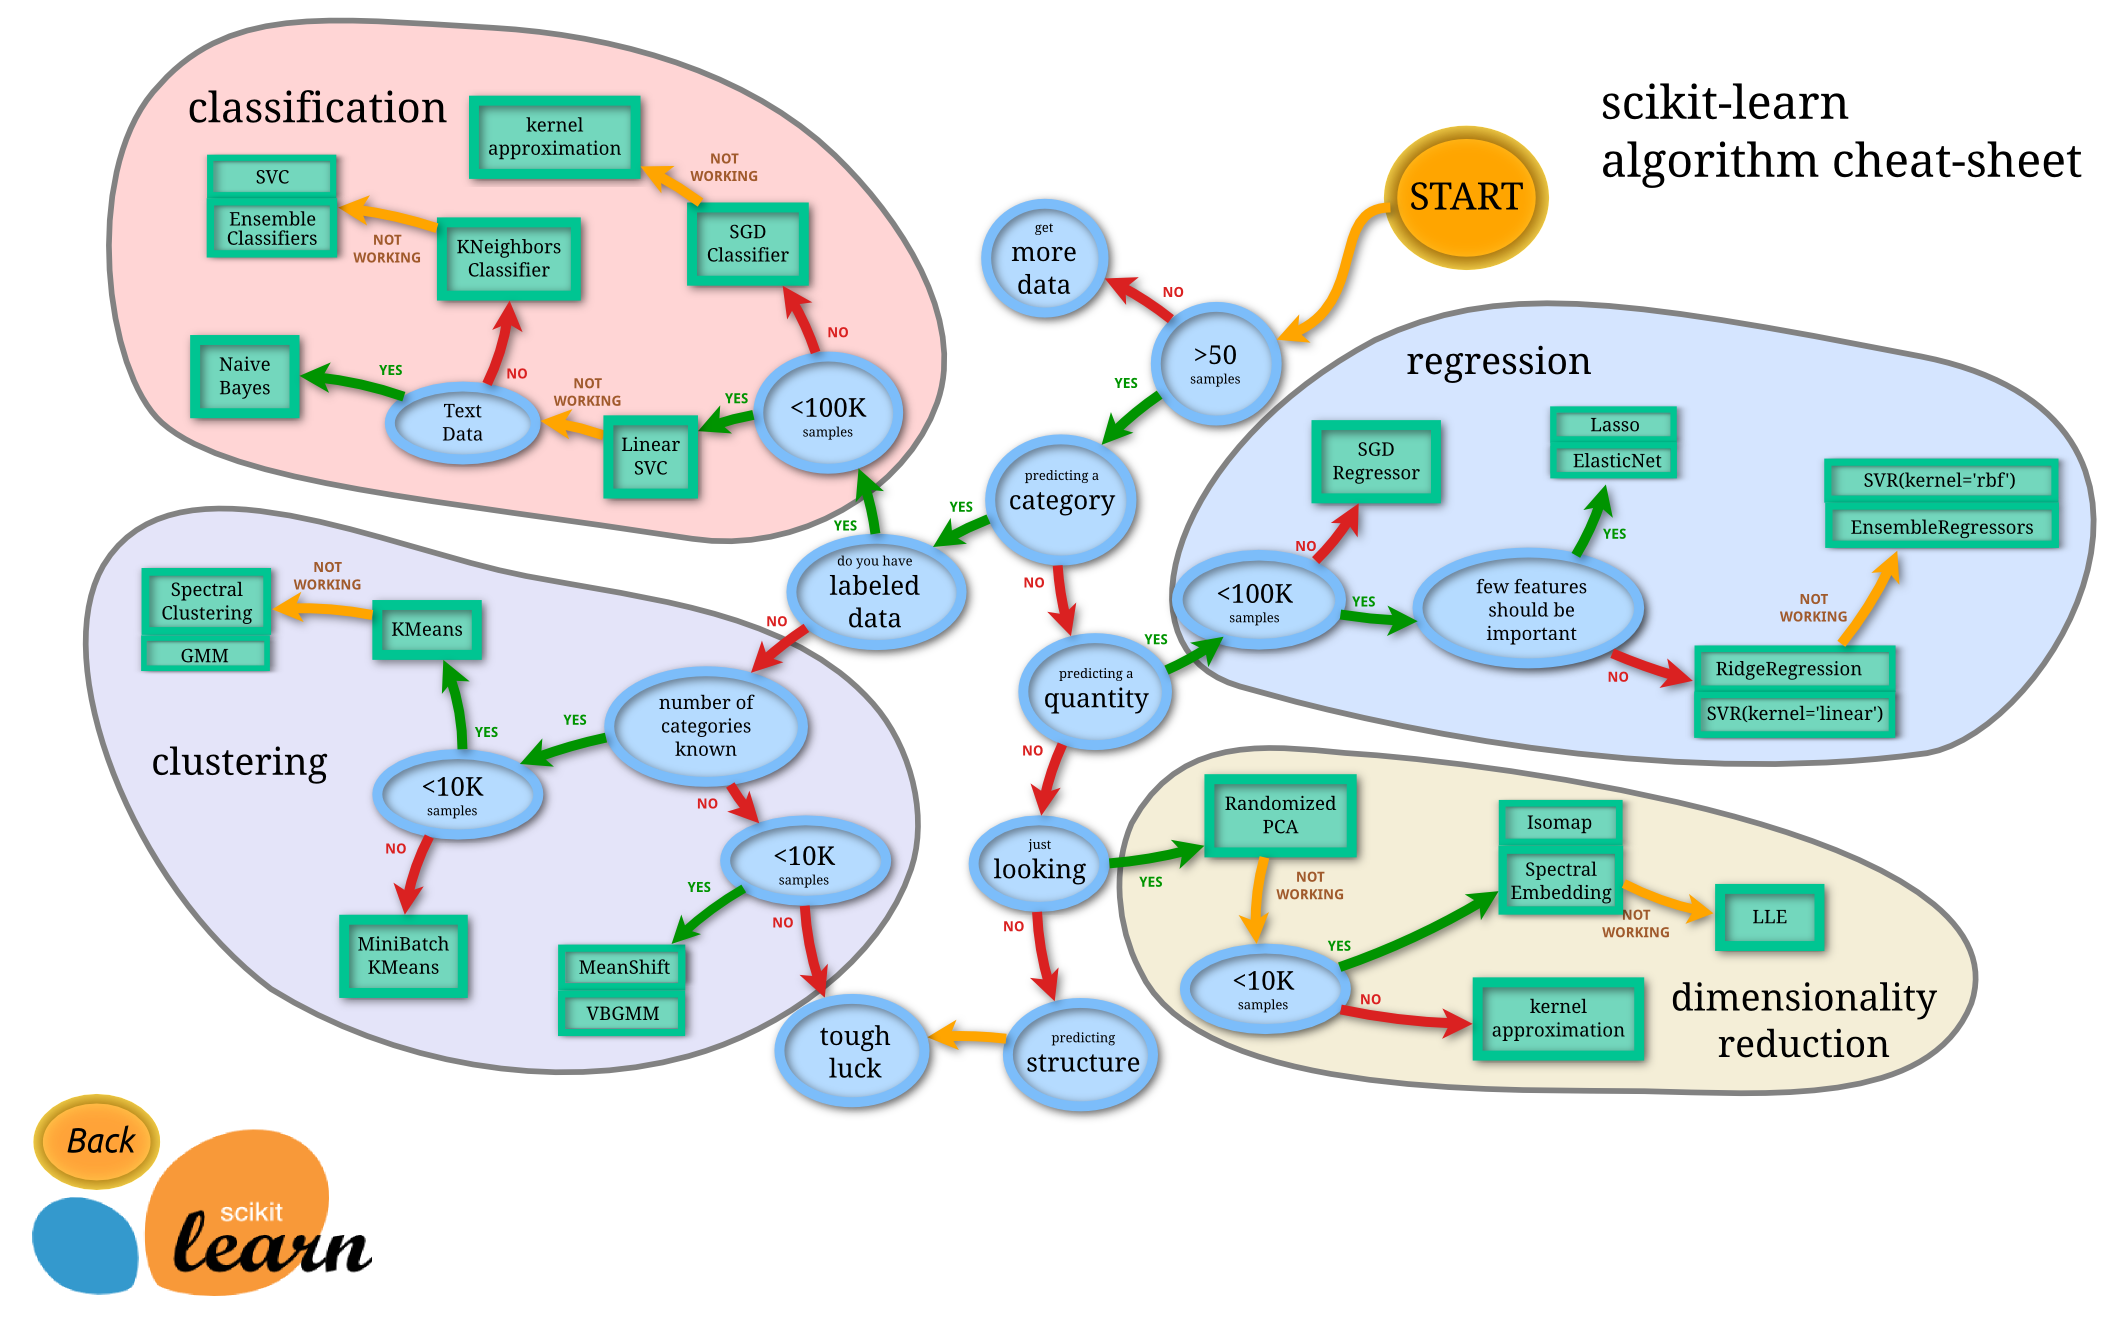
\includegraphics[width=\textwidth]{scheme_estimators.png}
	\caption{Esquema scikit-learn para la elección de un estimador}
	\label{fig:scheme_estimators}
\end{figure}


En nuestro caso contamos con más de 50 muestras, queremos predecir a que categoría pertenecen y contamos con los datos etiquetados gracias a la columna \textit{Attrition}.
Por tanto, nos encontramos en la burbuja \textit{classification} de la Figura \ref{fig:scheme_estimators}.
Y vamos a elaborar un proceso para decidir cual de ellos nos conviene más.\\

Para construir un modelo es necesario determinar las características que se van a usar, con que estimador se va a realizar la predicción y bajo que parámetros.

\subsection{Cálculo de la precisión de un modelo}
Una vez elegido el modelo existen distintas formas de evaluar dicho modelo. Esto es posible en problemas supervisados, como es nuestro caso en el que conocemos el resultado para ciertos datos.\\

Con el modelo elegido es necesario entrenarlo con un conjunto de datos. Si lo entrenamos con todos los datos con los que contamos, solo podremos realizar predicciones con muestras que pertenecen al conjunto de entrenamiento. Lo cual no es muy revelador, pues es normal que el modelo se comporte bien ante muestras con las cuales se le ha entrenado.\\

Para evitar caer en este error existe el método de separación de los datos en dos conjuntos, uno de entrenamiento y otro de pruebas. Este método es conocido como \textbf{Split Training}. Podemos ver esta separación en la Figura \ref{fig:splittraining}.\\

Este método consiste en separar los datos en dos conjuntos: uno de entrenamiento (\textit{train}), y otro de pruebas (\textit{test}).	
Se entrena al modelo con el conjunto de entrenamiento y se realiza la predicción con los datos de prueba. Una vez realizada la predicción se compara con el resultado correcto utilizando alguna sistema de puntuación (accuracy, f1, roc\_auc \ldots).


\begin{figure}[H]
\centering
\begin{tikzpicture}[every node/.append style={draw, rounded corners, inner sep=10pt}]
    \node [text width=3cm, text centered,rectangle split, rectangle split horizontal, rectangle split parts=2, rectangle split part fill={green!50, red!50}]
        {Training
		\nodepart{two} Test};
		 
\end{tikzpicture}
\caption{Split training}
\label{fig:splittraining}
\end{figure}

Sin embargo, puede que al hacer la separación en estos dos conjuntos se de un caso óptimo o por el contrario un caso fatal. Es por eso que se introduce otro nuevo método de evaluación, \textbf{Cross Validation} o Validación Cruzada.\\

Este método consiste en dividir los datos en una partición con $k$ conjuntos. Y realizar $k$ veces el método \textit{Split Training}. En cada iteración, el conjunto \textit{test} va siendo un elemento distinto de la partición y el conjunto \textit{train} lo forman los $k-1$ elementos restantes de la partición.
Una vez finalizadas cada una de las $k$ evaluaciones con \textit{Split training} se realiza la media de las puntuaciones obtenidas, dando lugar a la puntuación con \textit{Cross Validation}. Podemos ver un ejemplo en la Figura \ref{fig:crossvalidation}.


\begin{figure}
\centering
\begin{tikzpicture}
%[every node/.append style={draw, rounded corners, inner sep=10pt}]
\tikzset{
	block/.style={
		draw, rounded corners, inner sep=10pt,	
       text width=3cm, text centered,rectangle split, rectangle split horizontal, rectangle split parts=3
       }
}

    \node [block, rectangle split part fill={red!50, green!50, green!50}] (uno)
        {Test
         \nodepart{two} Training
		 \nodepart{three} Training};
		 
	\node [block, below=1cm of uno, rectangle split part fill={green!50, red!50, green!50}] (dos)
        {Training
         \nodepart{two} Test
		 \nodepart{three} Training};
		 
	\node [block, below=1cm of dos, rectangle split part fill={green!50, green!50, red!50}] (tres)
        {Training
         \nodepart{two} Training
		 \nodepart{three} Test};
		 
	\node[right=of uno] (num_uno){87\%};
	\node[right=of dos] (num_dos){92\%};
	\node[right=of tres](num_tres){88\%};
	\node[below=of num_tres] (num_total){89\%}
	(num_tres.south) -- coordinate (aux) (num_tres.south|-num_total.north);
	
	\draw ([xshift=-1cm]num_total.north west|-aux) -- ([xshift=1cm]num_total.north east|-aux);   
		 
\end{tikzpicture}
\caption{Evaluación con el método \textit{Cross Validation} con $k=3$}
\label{fig:crossvalidation}
\end{figure}


\subsection{Selección de características}
Esta fase consiste en la elección de aquellas características que aporten más información, para poder ser usadas en los distintos estimadores.
Una pregunta común sería, ¿Por qué no usamos todas las características para realizar la predicción? La respuesta es sencilla, y es que en este caso, más no significa mejor.
Usar características que no aportan información e introducen ruido en los datos repercute negativamente en la precisión del modelo.\\


La librería \textit{scikit-learn} proporciona mecanismos para la selección automática de características.
Estos son los que hemos usado:

\begin{itemize}
\item \textbf{Recursive Feature Elimination}. Dado un estimador que asigne pesos a las características RFE comienza con todas las características y recursivamente va considerando conjuntos más pequeños de características.
Si usamos la clase \texttt{sklearn.feature\_selection.RFECV} de \textit{scikit-learn} podemos realizar este proceso de eliminación encontrando el número óptimo de características.

\item \textbf{Feature selection}. Únicamente puede ser usado con estimadores que asigna importancia a las características tras ser entrenado. Podemos hacer uso de este método de selección de características gracias a la clase \texttt{sklearn.feature\_selection.SelectFromModel} de \textit{scikit-learn}.

\end{itemize}

\subsection{Optimización de parámetros}
Una vez elegido un estimador, es necesario configurar los parámetros para obtener el mejor resultado posible con dicho estimador. Para ello existe una clase en \textit{scikit-learn} llamada \texttt{sklearn.model\_selection.GridSearchCV} a la cual le podemos pasar como argumentos un diccionario de \textit{python} con los valores que debe explorar para cada uno de los parámetros del estimador. Y lo que hace \textit{gridSearchCV} es ejecutar \textit{Cross Validation} para las distintas combinaciones de parámetros.
Una vez finalizadas, podemos acceder tanto a la puntuación más alta como a los parámetros del estimador que han dado lugar a dicha puntuación.


\subsection{Selección del estimador}
Los diferente estimadores que he probado son:

\begin{itemize}
\item \textbf{Linear Support Vector Classification}. Perteneciente a la familia de estimadores \textit{lineales}, cuyo objetivo es la construcción de un hiperplano en el espacio donde se encuentran los datos. De manera que un punto se clasificará dependiendo de a que lado del hiperplano se encuentre.

\item \textbf{K-vecinos más cercanos o K nearest neighbors Classifier}. Este estimador tiene como parámetros un valor $k$ que indica el número de vecinos en los que debe fijarse y otro parámetro \textit{weight\_options} que puede tomar los valores \textit{uniform} y \textit{distance}.
A la hora de clasificar un punto el estimador se fija en los $k$ puntos de entrenamiento más cercanos, detecta que clase es la más común en esos $k$ puntos, y esa clase es el resultado de la predicción. Cuando el parámetro \textit{weight\_options} tiene el valor \textit{distance} se ponderan los valores de los $k$ vecinos con el inverso de la distancia al punto que deseamos clasificar.

\item \textbf{Regresión logística} se trata de un tipo de análisis de regresión usado para predecir el resultado de una variable categórica.

\end{itemize}


El resultado de todo el proceso ha dado lugar al modelo formado por el estimador Regresión logística, con las características obtenidas tras aplicar el método de \textit{Recursive Feature Elimination}. Resultando ser 42 el número óptimo de características.\\

La búsqueda de los parámetros con \textit{GridSearchCV} ha dado lugar a la siguiente configuración.\\

%['OverTime_Yes', 'YearsAtCompany', 'JobInvolvement', 'JobLevel', 'JobSatisfaction', 'NumCompaniesWorked', 'BusinessTravel_Travel_Rarely', 'BusinessTravel_Travel_Frequently', 'Department_Research & Development', 'Department_Sales', 'EducationField_Life Sciences', 'EducationField_Marketing', 'EducationField_Medical', 'EducationField_Other', 'EducationField_Technical Degree', 'EnvironmentSatisfaction', 'Gender_Male', 'JobRole_Human Resources', 'JobRole_Laboratory Technician', 'JobRole_Manager', 'JobRole_Manufacturing Director', 'JobRole_Research Director', 'JobRole_Research Scientist', 'JobRole_Sales Executive', 'JobRole_Sales Representative', 'MaritalStatus_Single', 'MaritalStatus_Married', 'PerformanceRating', 'RelationshipSatisfaction', 'StockOptionLevel', 'TrainingTimesLastYear', 'WorkLifeBalance', 'YearsInCurrentRole', 'YearsSinceLastPromotion', 'YearsWithCurrManager', 'Age_Over', 'Income_Over', 'Distance_Over', 'AtCompany_Over', 'OverTime_Balance', 'YearsPerCompany', 'YearsAtCurrRole_Rate']

\begin{lstlisting}[language=python, breaklines]
	LogisticRegression(penalty= 'l2',C=1, fit_intercept=True, intercept_scaling=0.1, tol=0.001, class_weight=None)
\end{lstlisting}

Proporcionando una precisión de 89,38 \%\\


Ahora que hemos elegido el modelo que vamos a usar para realizar las predicciones, tenemos que entrenarlo con todos los datos con los que contamos (con los 1470 empleados).
De modo que podremos realizar predicciones sobre datos que esten fuera de nuestra población inicial, teniendo el modelo entrenado lo máximo posible.\\










